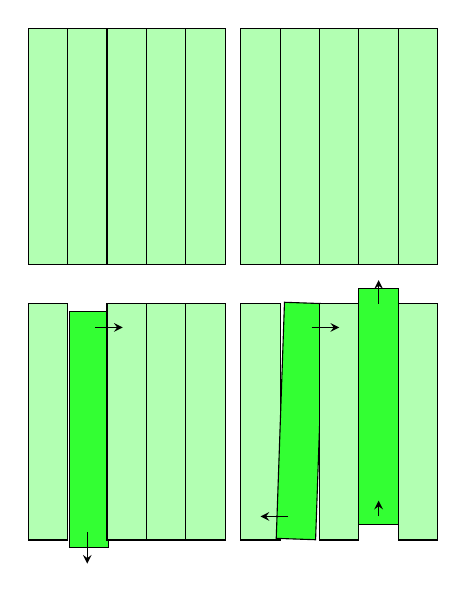
\begin{tikzpicture}
  % this is the ideal detector
  \node[rectangle,
      draw = black,
      % text = ,
      fill = green!30!white,
      minimum width = 0.5cm,
      minimum height = 3cm] (r) at (0,0) {};
  \node[rectangle,
      draw = black,
      % text = ,
      fill = green!80!white,
      minimum width = 0.5cm,
      minimum height = 3cm] (r) at (0.525,-0.1) {};
  \node[rectangle,
      draw = black,
      % text = ,
      fill = green!30!white,
      minimum width = 0.5cm,
      minimum height = 3cm] (r) at (1,0) {};
  \node[rectangle,
      draw = black,
      % text = ,
      fill = green!30!white,
      minimum width = 0.5cm,
      minimum height = 3cm] (r) at (1.5,0) {};
  \node[rectangle,
      draw = black,
      % text = ,
      fill = green!30!white,
      minimum width = 0.5cm,
      minimum height = 3cm] (r) at (2,0) {};

  \node[rectangle,
      draw = black,
      % text = ,
      fill = green!30!white,
      minimum width = 0.5cm,
      minimum height = 3cm] (r) at (2.7,0) {};
  \node[rectangle,
      draw = black,
      % text = ,
      fill = green!80!white,
      rotate around = {-2:(3.2,0)},
      minimum width = 0.5cm,
      minimum height = 3cm] (r) at (3.2,-0.1) {};
  % \draw (2.7,0) -- (5.7,0);
  \node[rectangle,
      draw = black,
      % text = ,
      fill = green!30!white,
      minimum width = 0.5cm,
      minimum height = 3cm] (r) at (3.7,0) {};
  \node[rectangle,
      draw = black,
      % text = ,
      fill = green!80!white,
      minimum width = 0.5cm,
      minimum height = 3cm] (r) at (4.2,0.2) {};
  \node[rectangle,
      draw = black,
      % text = ,
      fill = green!30!white,
      minimum width = 0.5cm,
      minimum height = 3cm] (r) at (4.7,0) {};

% now below it the physical detector
\node[rectangle,
    draw = black,
    % text = ,
    fill = green!30!white,
    minimum width = 0.5cm,
    minimum height = 3cm] (r) at (0,3.5) {};
\node[rectangle,
    draw = black,
    % text = ,
    fill = green!30!white,
    minimum width = 0.5cm,
    minimum height = 3cm] (r) at (0.5,3.5) {};
\node[rectangle,
    draw = black,
    % text = ,
    fill = green!30!white,
    minimum width = 0.5cm,
    minimum height = 3cm] (r) at (1,3.5) {};
\node[rectangle,
    draw = black,
    % text = ,
    fill = green!30!white,
    minimum width = 0.5cm,
    minimum height = 3cm] (r) at (1.5,3.5) {};
\node[rectangle,
    draw = black,
    % text = ,
    fill = green!30!white,
    minimum width = 0.5cm,
    minimum height = 3cm] (r) at (2,3.5) {};

\node[rectangle,
    draw = black,
    % text = ,
    fill = green!30!white,
    minimum width = 0.5cm,
    minimum height = 3cm] (r) at (2.7,3.5) {};
\node[rectangle,
    draw = black,
    % text = ,
    fill = green!30!white,
    minimum width = 0.5cm,
    minimum height = 3cm] (r) at (3.2,3.5) {};
\node[rectangle,
    draw = black,
    % text = ,
    fill = green!30!white,
    minimum width = 0.5cm,
    minimum height = 3cm] (r) at (3.7,3.5) {};
\node[rectangle,
    draw = black,
    % text = ,
    fill = green!30!white,
    minimum width = 0.5cm,
    minimum height = 3cm] (r) at (4.2,3.5) {};
\node[rectangle,
    draw = black,
    % text = ,
    fill = green!30!white,
    minimum width = 0.5cm,
    minimum height = 3cm] (r) at (4.7,3.5) {};

% draw arrows indicating the movement
% x and y translation
\draw [-stealth] (0.6,1.2) -- (0.95,1.2);
\draw [-stealth] (0.5,-1.4) -- (0.5,-1.8);

% rotation
\draw [-stealth] (3.35,1.2) -- (3.7,1.2);
\draw [-stealth] (3.05,-1.2) -- (2.7,-1.2);
% single translation
\draw [-stealth] (4.2,1.5) -- (4.2,1.8);
\draw [-stealth] (4.2,-1.2) -- (4.2,-1);

\end{tikzpicture}
